\section{Covariance between cities}
% As an extension to the project we decided to investigate the correlation between two different cities, with possibly a time lag. To this end we implement an extra function into our \texttt{tempTrender} object. This function takes as inputs a data path for another measuring station and then plots the correlation graph between the two stations. \\
%We now present some figures showing the correlation between different cites with different time lags

For our third result we wished to study the covariance of the temperature between different cities with possibly a time lag. We made use of three cities, Lund, Falsterbo and Umeå. The covariance $Cov(X,Y)$ of two real-valued random variables $X, Y$ is formally defined as $Cov(X,Y) = E((X-E(X))(Y-E(Y))$, where $E(X)$ is the expectation of $X$. Intuitively, or as an interpretation, the covariance tells us how $X$ and $Y$ relate to each other, that is, it is the degree by which the random variables change with respect to each other. 

The way we did this was by implementing an extra function into our \texttt{tempTrender} object. This function takes as inputs a data path for another measuring station and then plots the covariance between the two. 

We show some figures of the covariance between Lund and Falsterbo. Further we show the covarriance between  Lund at different time lags.


\begin{figure}[h]
    \centering
    \begin{subfigure}[b]{0.49\textwidth}
    \centering
    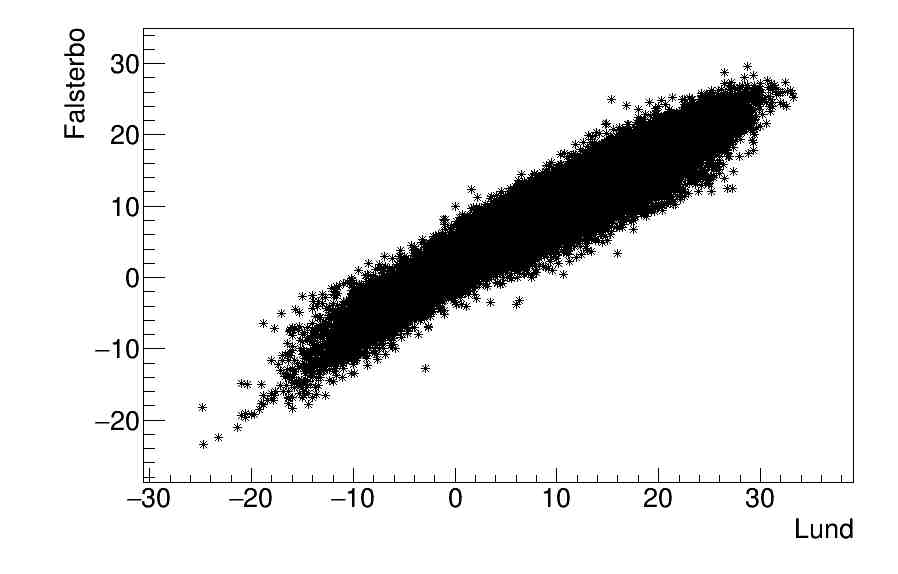
\includegraphics[width=\textwidth]{LU_FAL_E.jpg}
        \caption{Covarriance between Lund and Falsterbo}
    \end{subfigure}
    \hfill
    \begin{subfigure}[b]{0.49\textwidth}
    \centering
    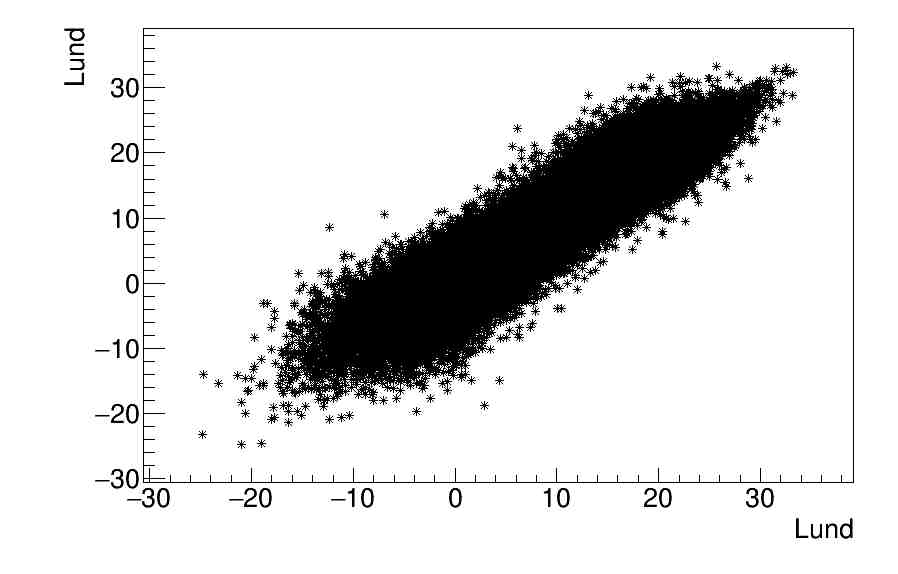
\includegraphics[width=\textwidth]{LU_LU_1D_E.jpg}
        \caption{Lund with time lag 1 Day}
    \end{subfigure}
    
    \begin{subfigure}[b]{0.49\textwidth}
    \centering
    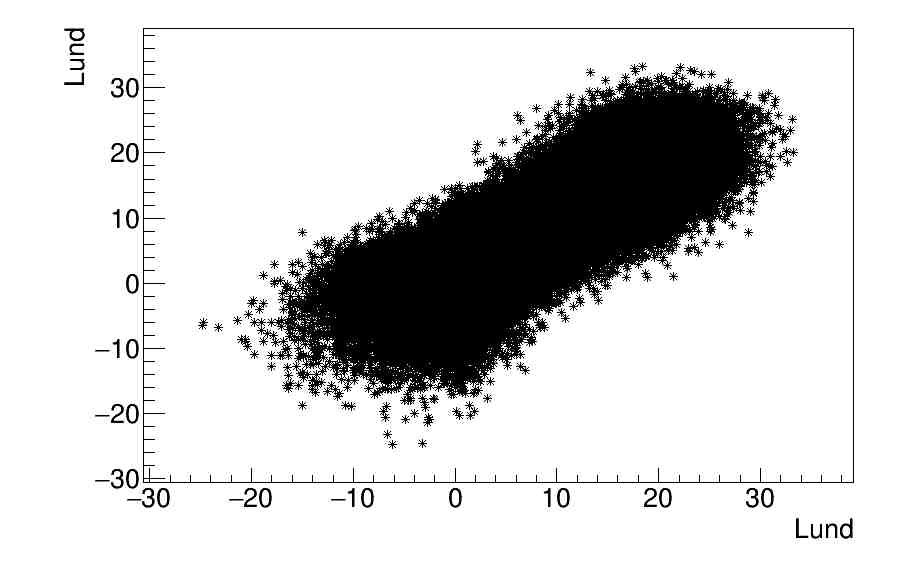
\includegraphics[width=\textwidth]{LU_LU_1W_E.jpg}
        \caption{Lund with time lag 1 Week}
    \end{subfigure}
    \hfill
    \begin{subfigure}[b]{0.49\textwidth}
    \centering
    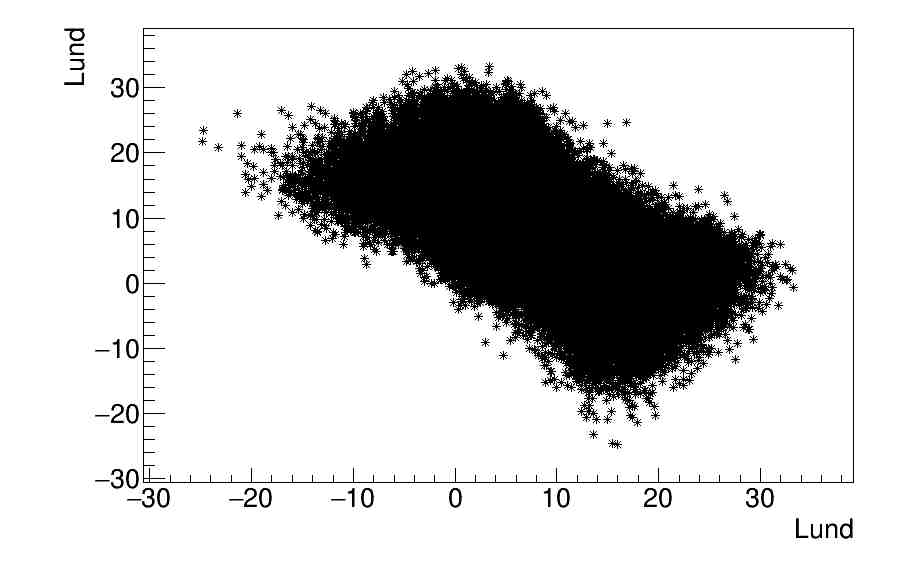
\includegraphics[width=\textwidth]{LU_LU_6M_E.jpg}
        \caption{Lund with time lag 6 Months}
    \end{subfigure}
\end{figure}

Due to the close proximity of Lund and Falsterbo we expected the covariance for Lund and Falsterbo to be fairly good. Further we should see a better correlation in the graphs with a time lag with 1 day than 1 week, while the 6 months time lag should have very week negative correlation which we see. 

\newpage